\documentclass{article}
\usepackage[utf8]{inputenc}
\usepackage{graphicx}
\usepackage{flafter}
\usepackage{float}
\usepackage{subcaption}
\graphicspath{ {./images/} }
\usepackage{minted}
\usepackage{hyperref}
\hypersetup{
    colorlinks=true,
    linkcolor=blue,
    filecolor=magenta,      
    urlcolor=cyan,
}
\urlstyle{same}

\title{Real-Time Options Pricing Model}
\author{Jaisal Friedman}
\date{December 16 2018}
\begin{document}
\maketitle


\begin{abstract}
    This paper explores the Black-Scholes-Merton options pricing model, derives a predictive extension model, and visualizes both models in comparison to real-time pricing options pricing. The paper also explores various methodologies of calculating historical volatility. A portfolio of 5 U.S. Market Stocks and 1 index fund was taken as example for the project. The model was limited to visual analysis from real-time simulations as further explained in the extensions section. 
\end{abstract}


\section{Introduction}
\begin{flushleft} The impact of the Black-Scholes-Merton model on modern financial markets drove the paper's initial fascination. The paper intends to visually model the Black-Scholes-Merton Model, a predictive extension model, and the real-time options spread for a better understanding of the options market. This project first seeks to explore the dynamics of the Black-Scholes-Merton and its derivation. The paper then introduces a predictive extension to which a visual analysis is displayed in real-time for one to decipher its effectiveness. Four methodologies for the historical volatility calculation were explored and compared in real-time between the 6 example assets. The Black-Scholes-Merton calculation for real-time assets with historical data was then modeled. The extended predictive model was derived for real-time assets. And lastly, the F-B-S, predictive model, and real-time options pricing was visually displayed and analyzed using 3D volatility surfaces. The paper, itself, will begin with the methodology: where the historical volatility calculations, assumptions of the Black-Scholes-Merton model, and the predictive extension will be discussed. Then introduce the implementation: where the real-time numerical simulation, 3D visualization, and discussion of results are presented. Lastly, it will conclude with a short conclusion, explanation of the software development, limitations, and possible extensions and improvements of the model.
\end{flushleft}


\section{Methodology}

\subsection{Introduction to the Black-Scholes-Merton Model}
\begin{flushleft}
The Black-Scholes model was initially published in 1973. It provided the first deterministic pricing model for the options market. This led to a boom in the options financial markets that has continued till present day. In 1976, Merton published his extension of the Black-Scholes model which included the effect of dividend payouts. Today, the Black-Scholes-Merton model is used to determine the Greeks and Implied Volatility in the financial options market. Its impact on efficiently pricing the options market as a benchmark model holds strong even some 40 years later. For this reason, this paper starts its extension and comparative visualization with such a model. 
\end{flushleft}
\subsection{Black-Scholes-Merton Equation}
\begin{flushleft}
$C_t(s,t) = S \cdot e^{-qt}  \cdot N (d_1) - X\cdot e^{-rt} \cdot N(d_2)$
\newline\newline
$P_t(S,t) = -e^{-qt}  \cdot  S \cdot N (-d_1) + X\cdot e^{-rt} \cdot N(-d_2)$
\newline\newline
where: 
\newline\newline
$d_1 = \frac {ln(\frac{S}{X}) + (r-q+ \frac{\sigma^2}{2}) \cdot t}{\sigma \cdot \sqrt {t}}$
\newline\newline
$d_2 = d_1 - \sigma \cdot \sqrt{t}$
\newline\newline
$N(x) = \int_{-\infty}^{x} {\frac {1}{\sqrt{2\pi}\cdot \sigma^2}\cdot e ^{\frac{-(u-\mu)^2}{2\sigma^2}} du},$
where $\sigma^2 = 1, \mu = 0$
\end{flushleft}

\subsubsection {Notable Assumptions}
\begin{flushleft}
\begin{enumerate}
\item The cumulative distribution function N(x) follows market probabilities. In fact, there are unpredictable Black Swan events which severely skew market movements. Fat Tail distributions are more accurate for financial markets. 
\item  Market speculation has no effect on the pricing of options.
\item The option is a European option meaning it can only be exercised at expiry. This makes the mathematics infinity more simple. However, for American options this is false; they can be executed at any moment. 
\end{enumerate}

\end{flushleft}

\subsubsection {Historical Volatility $\sigma$}
\begin{flushleft} Historical volatility in the Black-Scholes-Merton $\sigma$ can be calculated by different methods. Classically, $\sigma$ is calculated by either the standard deviation of the log returns or the percent change of close-to-close asset pricing for the past 30 days normalized to the last trading year. This methodology utilizes the close-to-close historical pricing. The log returns is argued to be a more mathematically sound indicator than percent change for $\sigma$. 
\newline \newline
$hv_{percent} = \sqrt{\frac{1}{N-1} \sum_{i=1}^N (x_i - \overline{x})^2},$ where $x=\frac{s(t)_{close} - s(t-1)_{close}}{s(t-1)_{close}} $
\newline\newline
$hv_{log} = \sqrt{\frac{1}{N-1} \sum_{i=1}^N (x_i - \overline{x})^2},$ where $x=log{\frac{S^t_{close}}{ S^{t-1}_{close}}}$
\end{flushleft}
\begin{flushleft} However, Historical volatility in the Black-Scholes-Merton $\sigma$ can also be calculated by intraday methods. This paper presents two possible extensions. The first is self-derived. It utilizes both the open-close and high-low pricing to return a weighted intraday historical volatility. The second is the highly referenced Parkinson Historical Intraday volatility calculation. Both methodologies utilizes the intraday historical pricing and provide a different outlook at on $\sigma$. 
\newline \newline
$hv_{w_ext} = \sqrt{\frac{1}{N-1} \sum_{i=1}^N (x_i - \overline{x})^2},$ where $x=log{\frac{S^t_{high}}{ S^{t-1}_{low}}} \cdot w + log{\frac{S^t_{high}}{ S^{t-1}_{low}}} \cdot (1-w)$
\newline\newline
$hv_{w_park} = \sqrt{\frac{1}{N} \sum_{i=1}^N \frac{1}{4\ln(2)}(x_i )^2},$ where $ x=log{\frac{S^t_{high}}{ S^{t-1}_{low}}} \cdot $
\end{flushleft}

\subsection{Predictive Extension}
\begin{flushleft}
The predictive extension presented in this paper builds off the Black-Scholes-Merton model. The model attempted to scale the B-S-M model by sigmoid function encapsulating current financial market health and beta exposure of the underlying asset to the market conditions.
\end{flushleft}

\subsubsection{Equation}
$M(c_1, c_2, dd, \beta, t) = \frac{x}{1+ (|x|)} + 1,$ where $x = \frac{c_1\beta\sqrt{t}}{dd} - c_2$
\newline\newline
$C_{ext}(s,t) = S \cdot e^{-qt}  \cdot N (d_1) - X\cdot e^{-rt} \cdot N(d_2) \cdot M(c_1, c_2,dd, \beta, t)$
\newline \newline
$P_{ext}(S,t) = (-e^{-qt}  \cdot  S \cdot N (-d_1) + X\cdot e^{-rt} \cdot N(-d_2)) \cdot \frac{1}{M(c_1, c_2,dd, \beta, t)}$
\newline \newline
where $c_1, c_2$ = constants, dd = defaulted debt and $\beta$ = risk exposure of an asset to the market
\newline
\subsubsection {Notable Assumptions}
\begin{flushleft}  
\begin{enumerate}
\item  Speculation about the current market conditions has an impact on the pricing of long-dated options. 
\item The $\beta$ exposure of an underlying asset to the market affects the pricing of certain assets over assets with a lower $\beta$. 
\item The time of the options has a square-root proportionality with the pricing of options under certain market conditions. Longer-dated options will be square-root proportionally more affected by overall market speculation. 
\item The dd, defaulted debt, indicator can be effectively represent the overall financial market health. 
\item The M function follows a Sigmoid proportionality with the Black-Scholes pricing model centered by $c_1, c_2$. 
\end{enumerate}
\end{flushleft}

\subsection {Real-Time Pricing}
\begin{flushleft} 
The real-time pricing involved a substantial amount of software development. This was deemed worthy as the model's visual analysis is better implemented in real-time. 
\end{flushleft}
\subsubsection {Assets Chosen}
\begin{itemize}
\item MSFT - Microsoft
\item BA - Boeing
\item V - Visa 
\item AAPL - Apple
\item GOOGL - Alphabet Class A
\item SPY -  SPDR S&P 500 ETF Trust
\end{itemize}
\begin{flushleft} 
These assets were chosen directly from my personal portfolio as they held the most interest to me. In the code, one can select their own portfolio assets to visualize. 
\end{flushleft}
\subsubsection {API Interactions}
\begin{enumerate}
\item FRED - Federal Reserve Economic Data
\item IEX Exchange - Real-time Stock Data 
\item Tradier - Real-time Options Data
\item Plotly - Interactive 3D Visualizations
\end{enumerate}
\newpage


\section{Implementation}
\subsection{Historical Volatility $\sigma$}
\begin{flushleft}
The implementation of the methodology was carried out in python. A working model was built to take real-time data and generate the appropriate visualization. 
\begin{minted}{python}
def hv_log(historicals, portfolio):
    dates = historicals['date']
    df = {}
    for stock in portfolio:
        sigmas = {}
        h = historicals[stock].join(dates)
        i = timedelta(days = 31)
        j = 1
        while(i+dates[j] <= dates[len(dates)-1]):
            h1 = h[(h['date'] >= dates[j-1]) & (h['date'] <= i+dates[j])]
            h1['volatility'] = h1['close'].pct_change()
            h1[1:]
            sigma_matrix = np.std(h1['volatility'])* np.sqrt(252)
            sigmas[i+dates[j]] = sigma_matrix
            j+=1
        df[stock] = sigmas
    return pd.DataFrame(df)
\end{minted}
\end{flushleft}

\subsection{Strike Prices}
\begin{flushleft}
Strike prices were calculated for each stock instead of scraped. 
\begin{minted}{python}
def strikes_(s, num):
    strikes = {}
    for ticker in s:
        if (s[ticker]>300):
            strikes[ticker] = [((round(s[ticker],-1))+((i-num)*10)) for i in range(2*num)]
        else:
            strikes[ticker] = [((round(s[ticker],-1))+((i-num)*5)) for i in range(2*num)]
    return strikes
\end{minted}
\end{flushleft}

\subsection{Expiration}
\begin{flushleft}
Expiration was also calculated for each stock. This was tricky because options expire on the 3rd Friday of each quarter. Because the project focused on longer-dated options. The code generated expiries from the current date for the next 3 quarters, and then 2 half-years from then. Although the code works efficiently, not all stocks follow these dates. There were 3 exceptions with the case examples which the Tradier library caught later. These had to manually fixed in Jupyter. 
\begin{minted}{python}
def third_friday(month, year):
    monthcal = c.monthdatescalendar(year, month)
    return monthcal[2][-1]
def generate_times(start, year, options_dates):
    t = []
    for i in range(6):
        if (i < 3):
            t.append(third_friday(options_dates[(start+i)%len(options_dates)], (year + int((start+i)/len(options_dates)))))
        else:
            t.append(third_friday(options_dates[(start+i+(i-2))%len(options_dates)], (year + int((start+i+(i-2))/len(options_dates)))))
    return t
def t_(today, options_dates):
    t = []
    month = int(today.month-1 + today.day/third_friday(today.month, today.year).day) % 12
    if (month > 9):
        t = generate_times(0, today.year+1, options_dates)
    elif (month > 6):
        t = generate_times(3, today.year, options_dates)
    elif (month > 3):
        t = generate_times(2, today.year, options_dates)
    else:
        t = generate_times(1, today.year, options_dates)
    return t
\end{minted}
\end{flushleft}

\subsection{Options Pricing}
\begin{flushleft}
These are the options pricing functions that were used in Jupyter to calculate real-time pricing of each model. 
\begin{minted}{python}
def M_(c1, c2,default, beta, t):
    x = c1*beta*np.sqrt(t)/default - c2
    return x/(1+abs(x))+1
def call_(s, x, t, r, q, d1, d2):
    return s*math.exp(-q*t)*norm.cdf(d1)-x*math.exp(-r*t)*norm.cdf(d2)
def put_(s, x, t, r, q, d1, d2):
    return x*math.exp(-r*t)*(1-norm.cdf(d2)) - s*math.exp(-q*t)*(1-norm.cdf(d1))
def d1_(s, x, t, r, q, sigma):
    return (np.log(s/x)+(r-q+(np.power(sigma,2)/2)*t)) / (sigma*np.sqrt(t))
def d2_(d1, sigma, t):
    return d1 - sigma*np.sqrt(t)
\end{minted}
\end{flushleft}

\subsection{Model Extension Indicators}
\begin{flushleft}
The US High Yield Master 2 Option-Adjusted Spread was used for the defaulted rate in the extended model. This is an economic indicator from FRED, which tracks the percent of high-yield bond defaults in the US. See figure 7 for reference. 
\newline\newline
This was used for the following reasons: 
\begin{enumerate}
\item It has historically predated US financial market crashes. Check 2007 and 2001. 
\item It represents the most leveraged defaulted debt within the financial markets this paper is addressing. 
\end{enumerate}
The $\beta$ values were pulled from the IEXFinance API. $\beta$ is the historical risk of an asset to the market fluctuations. It can be calculated by a regression analysis between historical asset and market returns. The $\beta$ for the SPY should be close to 1, while more volatile stocks like GOOGL will be closer to 1.5. 
\end{flushleft}

\subsection{Results}
\begin{flushleft}
1. \textbf{Historical Volatility} \newline 
The figures section contains the plots for each historical volatility calculation. There are two plots which show all 4 calculations on one. This was done for BA and AAPL as examples. \newline\newline
2. \textbf{3D Volatility Surfances} The volatility surfaces for each stock and each call/put are displayed below in the Figures section. However, there are interactive figures available to explore. The link is referenced in the Appendix.  See Figure 8-18 in Appendix and 3D Surfaces in Appendix under Code Base. 
\newline\newline
\textbf{These can be seen at in the Appendix section under Figures}
\end{flushleft}
\newpage

\section{Conclusion}
\subsection{Discussion}
\begin{flushleft}{
\begin{itemize}
  \item \textbf{Historical Volatility} \newline
  \tabHorizontal Historical Volatility was presented by 4 different methodologies. After the visualization of these 4 methodologies; it became clear that the classical calculation $hv_log$ made the most sense for the longer-term options I was considering. The intraday calculations, although interesting, often hold volatility that the market would not consider influential in longer dated options. 
  \item \textbf{Black-Scholes-Merton Extension} \newline
  \tabHorizontal The Black-Scholes-Merton Extension as seen in the figures below often intersects the Black-Scholes-Merton model surface and the Real-time Spread surface. More so, the Extension favors time as a more defining parameter than the Black-Scholes-Merton or Spread models. It is impossible to evaluate the effectiveness of the extension model on predicatively pricing future options. Because the predictive model implies that the current market conditions will effect future prices of the options and thus both the current Spread and the Black-Scholes-Merton model may not reflect the true options pricing. This is further discussed in the Extensions section below. 
  \item \textbf{3D Volatility Surfaces} \newline
  \tabHorizontal The 3D Volatility Surfaces are a great tool to explore market inefficiencies in options pricing. As a definitive analysis it is difficult to evaluate the effectiveness of the models in pricing options without taking into affect the change is options prices between days. This is because the market may contain arbitrary inefficies on any given day. 
\end{itemize}
} 
\end{flushleft}

\subsection{Improvements}
\begin{flushleft} 
\begin{itemize}
  \item \textbf{3D Surfaces for each Historical Volatility} \newline
  \tabHorizontal This would be an effective and interesting improvement to visualize the effect of $\sigma$ calculations on the 3D volatility surfaces. 
  \item \textbf{Parameter sweep for $c_1,c_2$} \newline
  \tabHorizontal A Parameter sweep over $c_1, c_2$ would be a better measure to fit the extension to current real-time market spread pricing. This would need to done over-time to ensure that certain market conditions at a singular point in time don't dominate the sweep.  
\end{itemize}
\end{flushleft}

\subsection{Extensions}
\begin{flushleft} 
\begin{itemize}
  \item \textbf{Fixing the Improvements} \newline
  \tabHorizontal Fixing the listed Improvements in the above section would clarify a more applicable 3D volatility surface and thus model extension. This could be used to further evaluate the effectiveness of the model extension  
  \item \textbf{Back-Test} \newline
  \tabHorizontal A back-test to validate the model would be a key extension. There are several ways this could take place. For example, the extension could simply track the pricing each day of all three-models and present a visualization of how each fluctuates with the market. Or the back-test could trace a period of high-default like 2007 to understand how the model would price options and if this would be effective in the long-run. One could also take the approach of tracking pricing of the models when it would be purchased vs. when it would expire. This would need some more distilled thought, however. 
  \item \textbf{American Binary Options} \newline
  \tabHorizontal The Black-Scholes-Merton equation and thus its extension implies that the option will only be exercised at expiry. This is untrue of American options and thus could be optimized by using a Binary American options pricing model. 
  \item \textbf{Cumulative Distribution Function} \newline
  \tabHorizontal The Cumulative Normal Distribution Function which the Black-Scholes-Merton uses to imply probabilities of future pricing changes on the underlying asset may not be an optimal technique to model the financial markets. One could try a Multi-Fractal approach or a Fat-tails distribution which more heavily weights highly improbable events and lessens the likelihood of slightly improbable events. This has been shown to more accurately model probabilities of pricing changes in financial market. This could be included in the back-test to use historical market conditions as a benchmark for accurateness of the model extension. 
\end{itemize}
\end{flushleft}


\section{Appendix}
\subsection{References}
\subsubsection{Bibliography}

\begin{itemize}
\item Black, Fischer and Scholes, Myron, (1972), The Valuation of Option Contracts and a Test of Market Efficiency, Journal of Finance, 27, issue 2, p. 399-417, https://EconPapers.repec.org/RePEc:bla:jfinan:v:27:y:1972:i:2:p:399-417.
\item Black, Fischer. "The pricing of commodity contracts." Journal of financial economics 3.1-2 (1976): 167-179.
\item Spurgin, Richard B., and Thomas Schneeweis. "Efficient Estimation of Intra-day Volatility: A Methodof-Moments approach incorporating Trading Range." Financial Markets Tick by Tick (1999).
\item Taleb, Nassim. Dynamic hedging: managing vanilla and exotic options. Vol. 64. John Wiley & Sons, 1997.
\end{itemize}

\subsubsection{API References}
\begin{itemize}
\item FRED API - \url{https://research.stlouisfed.org/docs/api/fred/}
\item Tradier API - \url{https://developer.tradier.com/}
\item IEX Exchange API - \url{https://iextrading.com/developer/docs/#getting-started}
\item Plotly API - \url{https://plot.ly/python/}
\end{itemize}


\subsection{Code Base}
\begin{flushleft}
 The project was written in python. 
\begin{itemize}
\item Github -  \url{https://github.com/jaisal1024/options_realtime_modeling}
\item  Interactive Volatility Surfaces - \url{https://plot.ly/~jaisal1024/#/}
\end{itemize}
\end{flushleft}

\subsection{Figures}
\begin{figure}[h!]
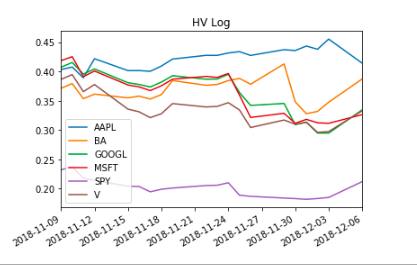
\includegraphics[width =\textwidth]{images/HV/HV-LOG.png}
\caption{Historical Volatility - Log}
\centering
\end{figure}
\begin{figure}[h!]
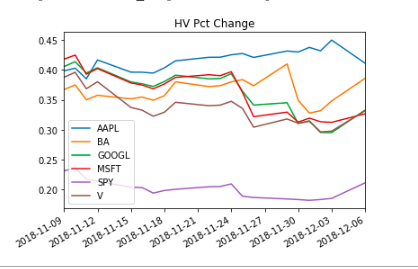
\includegraphics[width =\textwidth]{images/HV/HV-PCT.png}
\caption{Historical Volatility - Pct}
\centering
\end{figure}
\begin{figure}[h!]
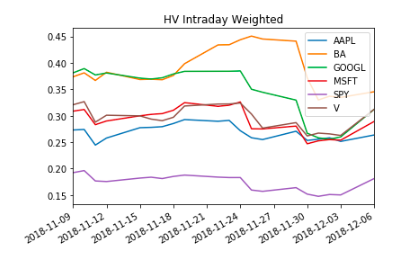
\includegraphics[width =\textwidth]{images/HV/HV_W.png}
\caption{Historical Volatility - Intraday Weighted}
\centering
\end{figure}
\begin{figure}[h!]
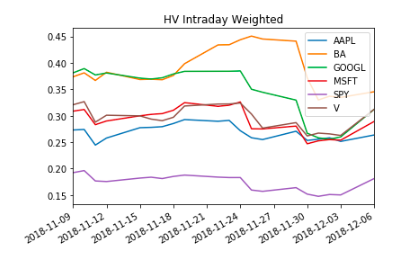
\includegraphics[width =\textwidth]{images/HV/HV_W.png}
\caption{Historical Volatility - Intraday Parkinson}
\centering
\end{figure}
\begin{figure}[h!]
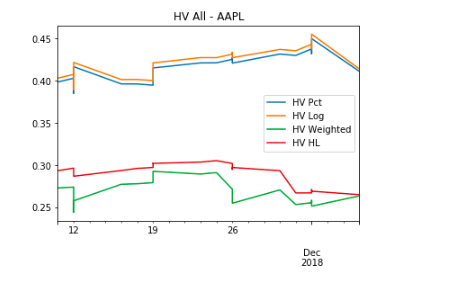
\includegraphics[width =\textwidth]{images/HV/HV-ALL-AAPL.png}
\caption{Historical Volatility - All APPL}
\centering
\end{figure}
\begin{figure}[h!]
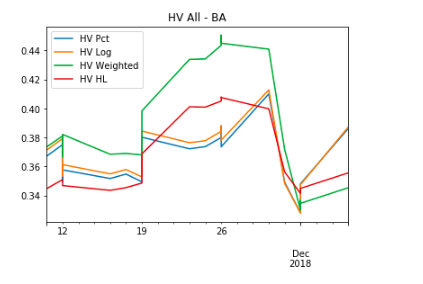
\includegraphics[width =\textwidth]{images/HV/HV-ALL-BA.png}
\caption{Historical Volatility - All BA}
\centering
\end{figure}

\begin{figure}[h!]
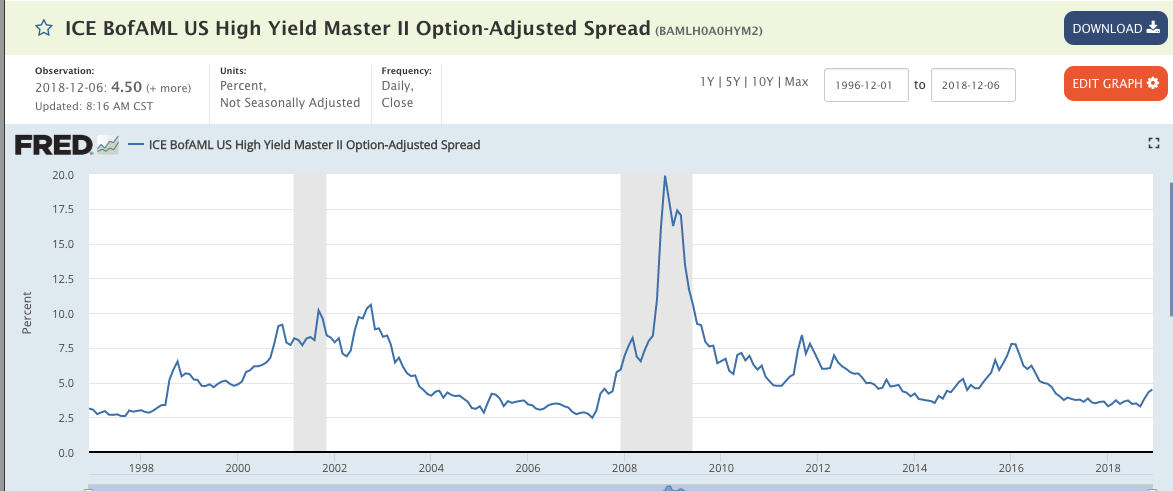
\includegraphics[width =\textwidth]{images/BAMF.png}
\caption{FRED Defaulted Debt Indicator}
\centering
\end{figure}


\begin{figure}[h!]
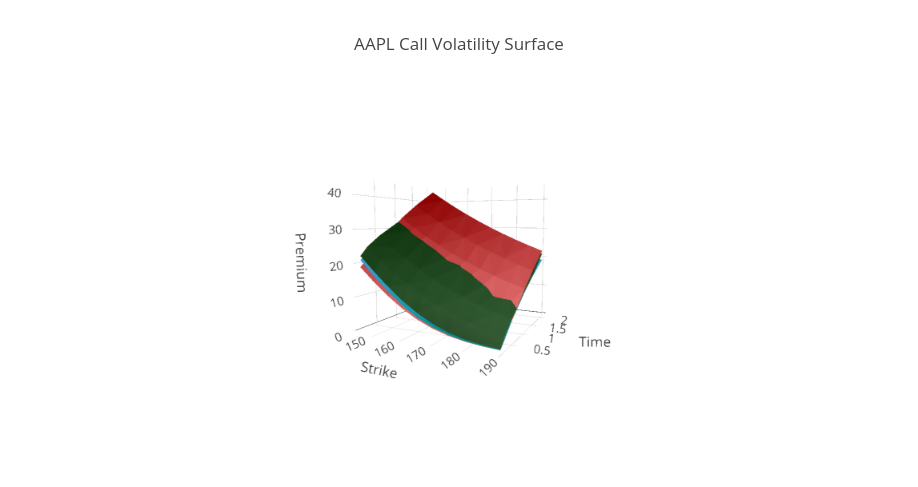
\includegraphics[width =\textwidth]{images/VolSurface/AAPLCall.png}
\caption{Apple Call Volatility Surface}
\centering
\end{figure}
\begin{figure}[h!]
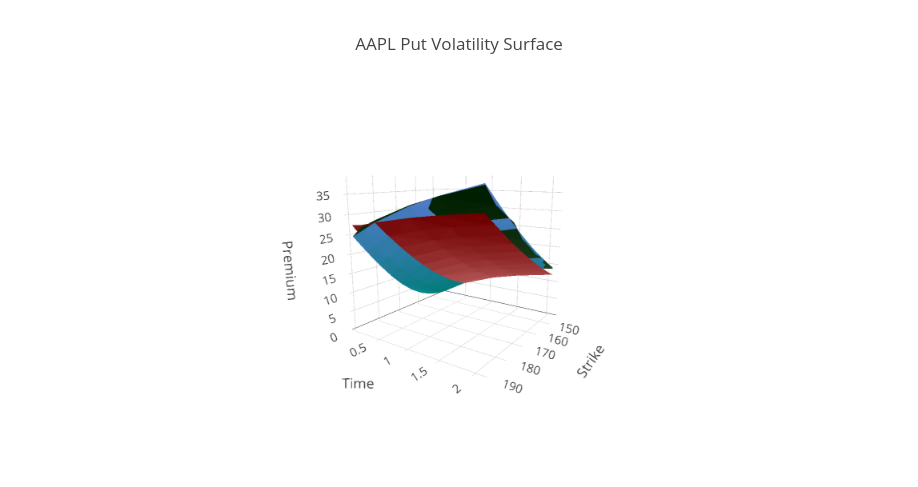
\includegraphics[width =\textwidth]{images/VolSurface/APPLPut.png}
\caption{Apple Put Volatility Surface}
\centering
\end{figure}
\begin{figure}[h!]
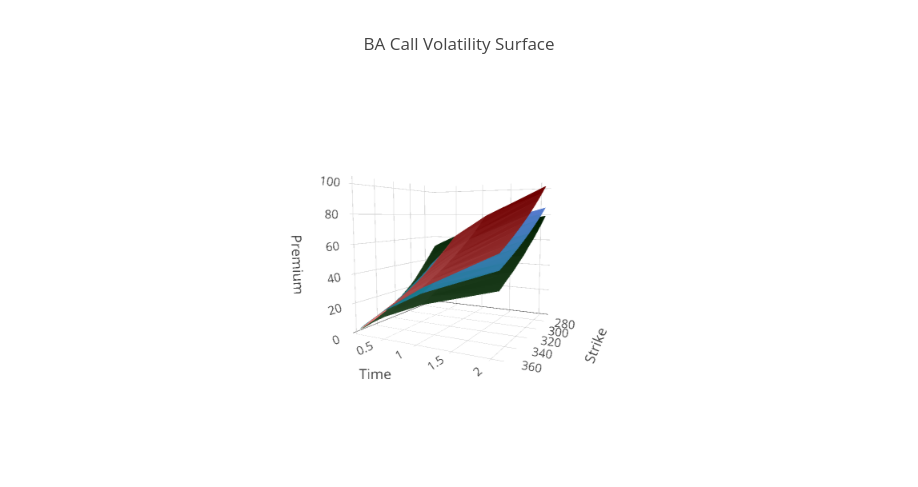
\includegraphics[width =\textwidth]{images/VolSurface/BACall.png}
\caption{Boeing Call Volatility Surface}
\centering
\end{figure}
\begin{figure}[h!]
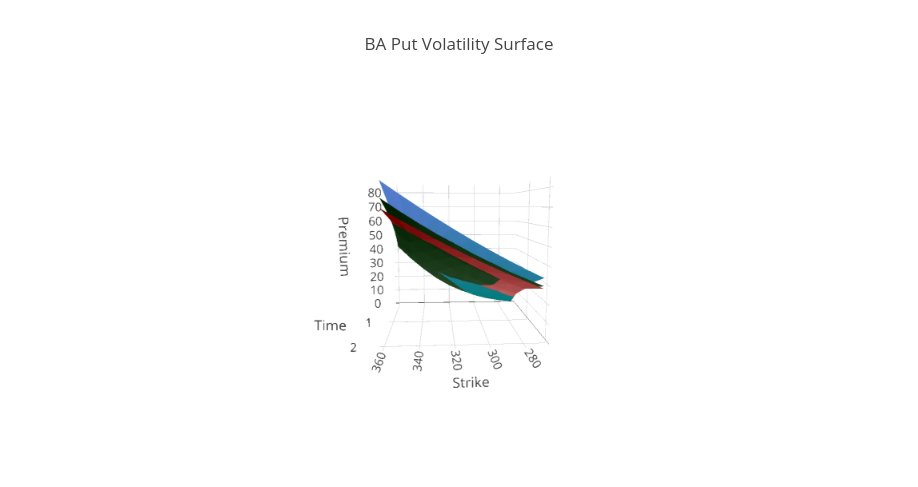
\includegraphics[width =\textwidth]{images/VolSurface/BAPut.png}
\caption{Boeing Put Volatility Surface}
\centering
\end{figure}
\begin{figure}[h!]
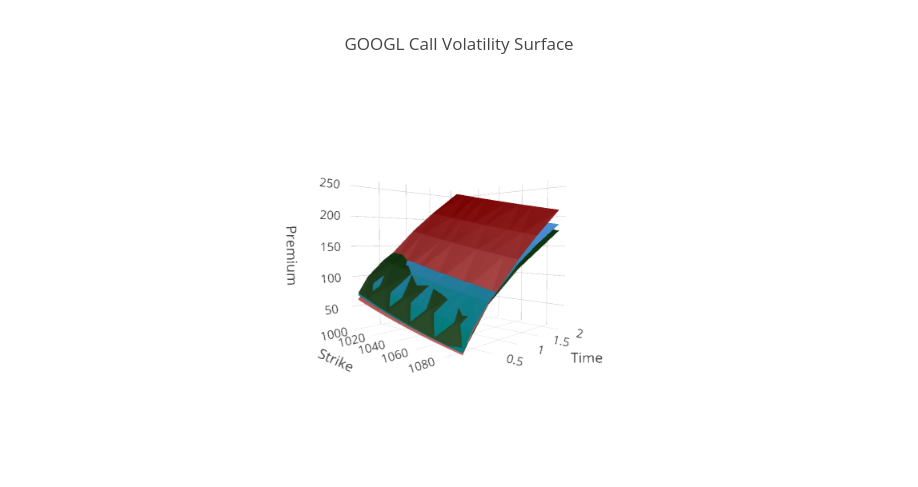
\includegraphics[width =\textwidth]{images/VolSurface/GOOGLCall.png}
\caption{Google Call Volatility Surface}
\centering
\end{figure}
\begin{figure}[h!]
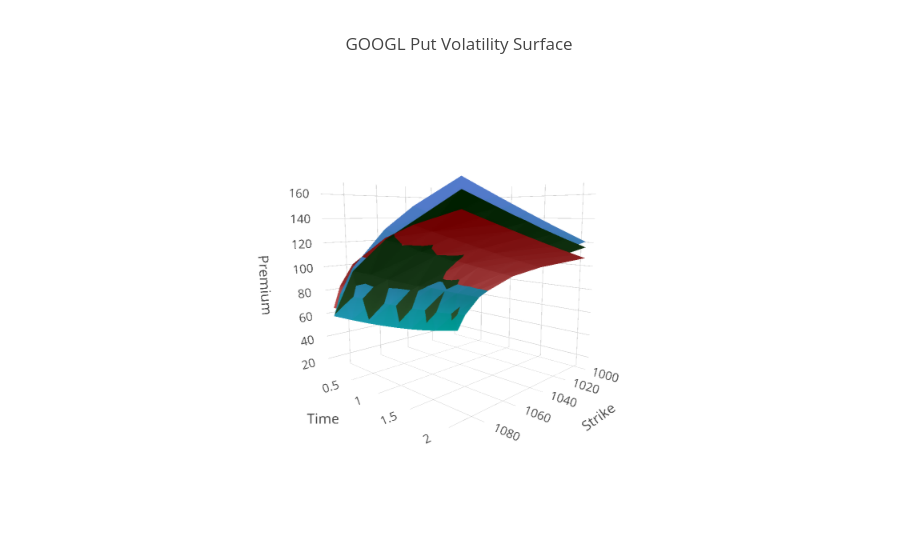
\includegraphics[width =\textwidth]{images/VolSurface/GOOGLPut.png}
\caption{Google Put Volatility Surface}
\centering
\end{figure}
\begin{figure}[h!]
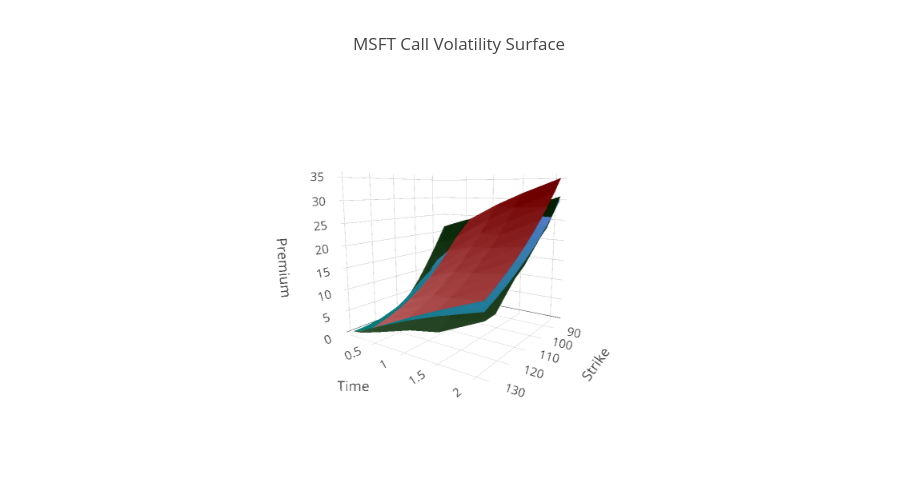
\includegraphics[width =\textwidth]{images/VolSurface/MSFTCall.png}
\caption{Microsoft Call Volatility Surface}
\centering
\end{figure}
\begin{figure}[h!]
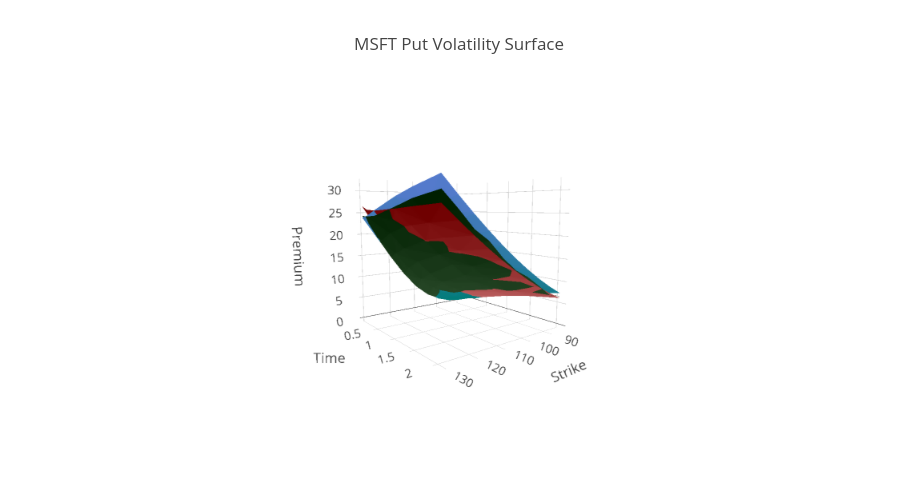
\includegraphics[width =\textwidth]{images/VolSurface/MSFTPut.png}
\caption{Microsoft Put Volatility Surface}
\centering
\end{figure}
\begin{figure}[h!]
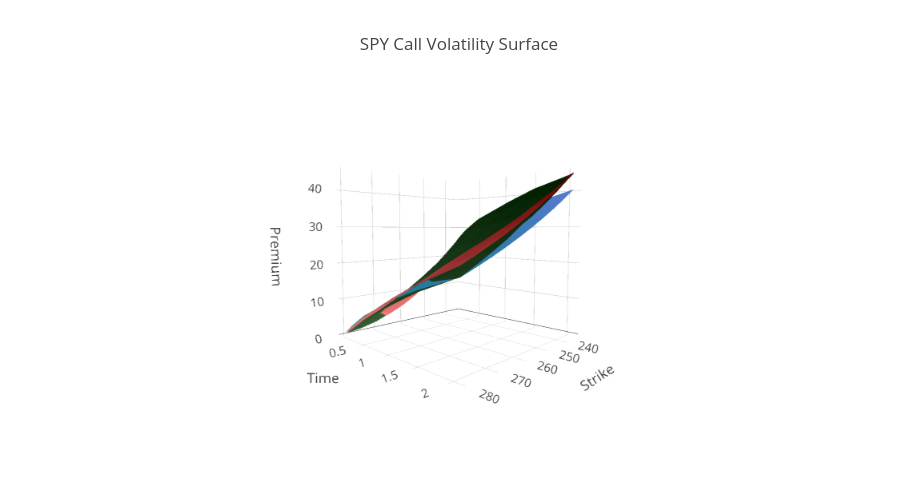
\includegraphics[width =\textwidth]{images/VolSurface/SPYCall.png}
\caption{SPY Call Volatility Surface}
\centering
\end{figure}
\begin{figure}[h!]
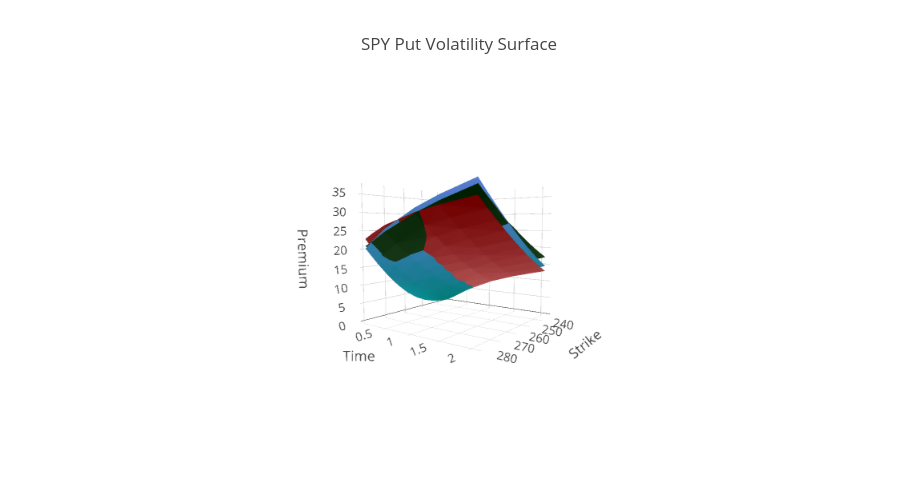
\includegraphics[width =\textwidth]{images/VolSurface/SPYPut.png}
\caption{SPY Put Volatility Surface}
\centering
\end{figure}
\begin{figure}[h!]
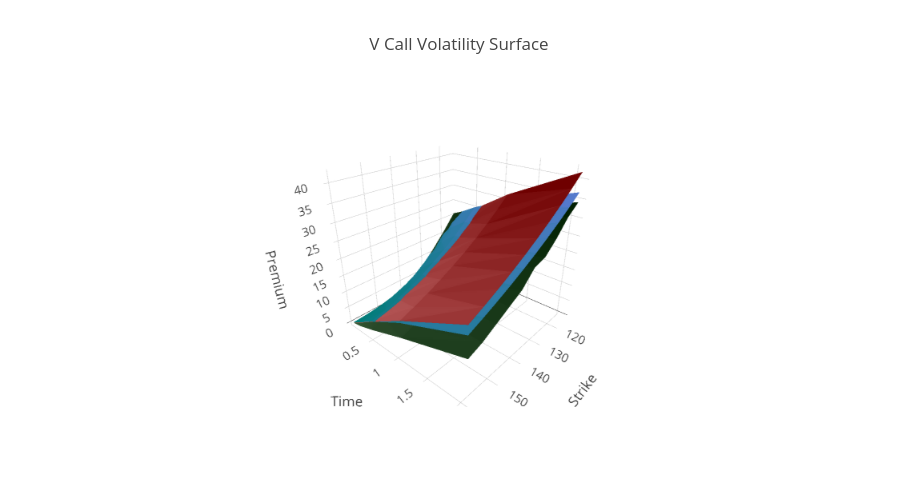
\includegraphics[width =\textwidth]{images/VolSurface/VCall.png}
\caption{Visa Call Volatility Surface}
\centering
\end{figure}
\begin{figure}[h!]
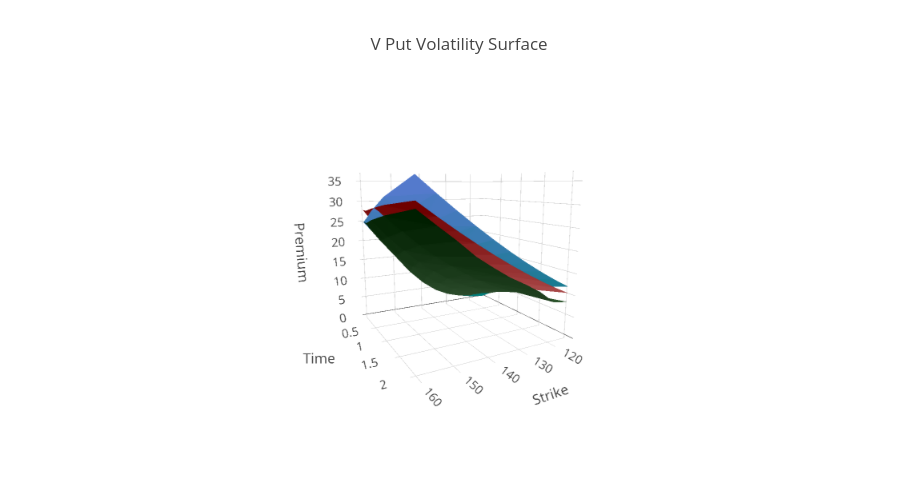
\includegraphics[width =\textwidth]{images/VolSurface/VPut.png}
\caption{Visa Put Volatility Surface}
\centering
\end{figure}


\end{document}
